\section{Hilfsmittel}
In dieser Arbeit wurden die folgenden Hilfsmittel genutzt:

\begin{itemize}
	\item Code-Editor: Intellij / TeXstudio
	\item Programmiersprachen: Java, TypeScript
	\item Datenbank: MySQL mit Testcontainers, H2
	\item Frameworks: Spring Boot, React
\end{itemize}

\clearpage

\section{Zusätzliche Abbildungen}

\begin{figure}[h]
	\centering
	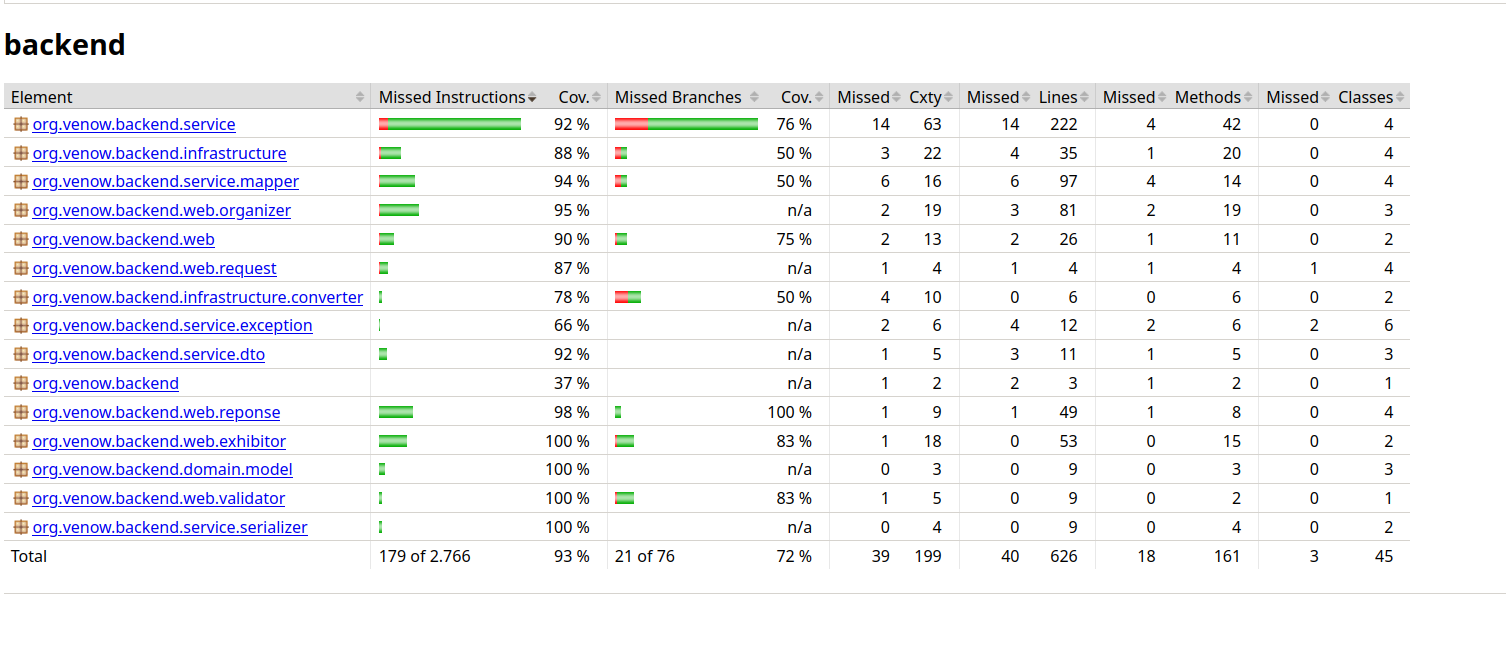
\includegraphics[width=1\textwidth]{fig/jacoco-honeycomb.png}
	\caption{Jacoco Honeycomb Testabdeckung}
	\label{fig:jacoco-honeycomb-full}
\end{figure}

\begin{figure}[h]
	\centering
	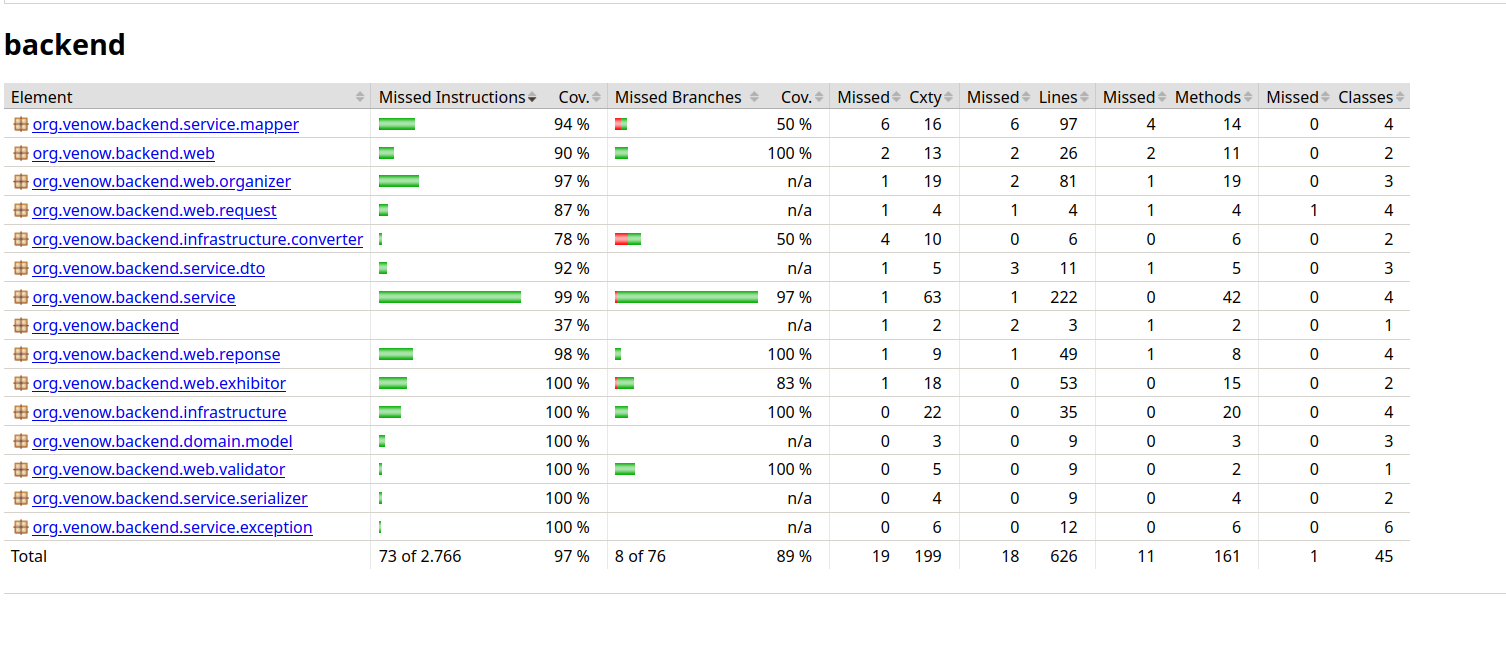
\includegraphics[width=1\textwidth]{fig/testpyrami-jacoco.png}
	\caption{Jacoco Testpyramid Testabdeckung}
	\label{fig:jacoco-testpyramid-full}
\end{figure}
\begin{figure}[h]
	\centering
	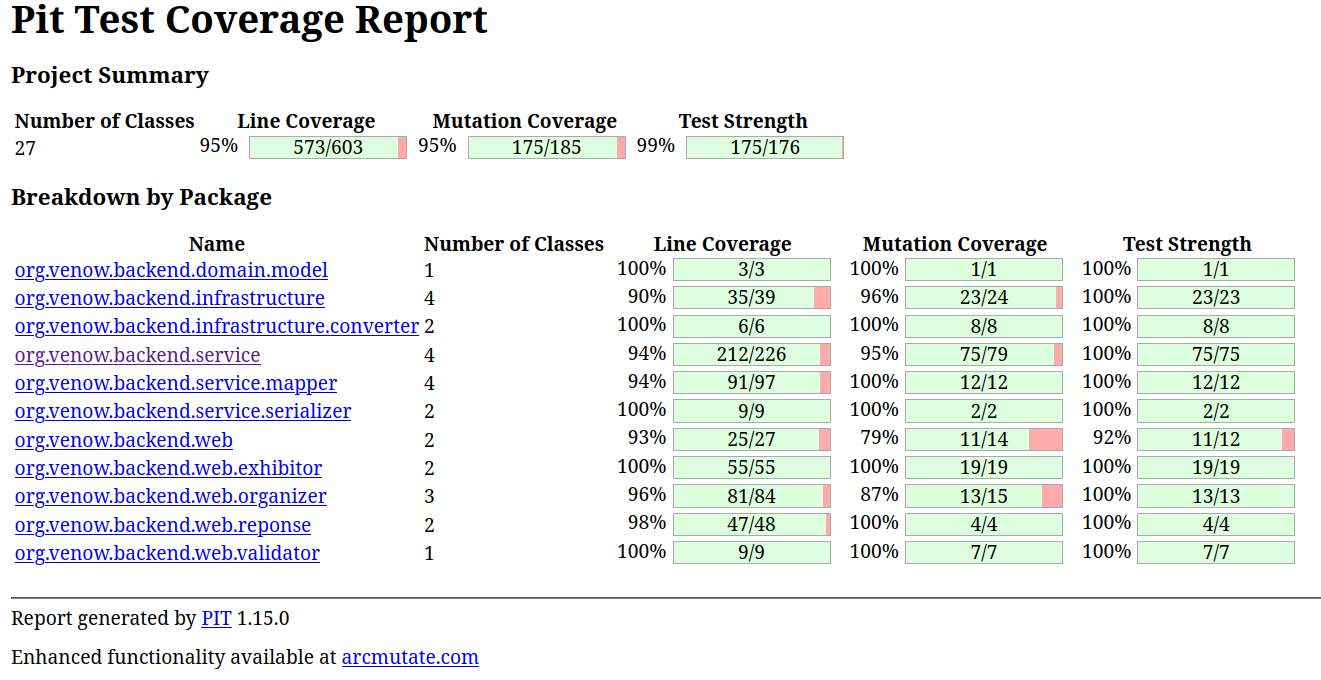
\includegraphics[width=1\textwidth]{fig/pitest-honeycomb.png}
	\caption{PIT - Mutation Honeycomb }
	\label{fig:pitest-honeycomb-full}
\end{figure}
\begin{figure}[h]
	\centering
	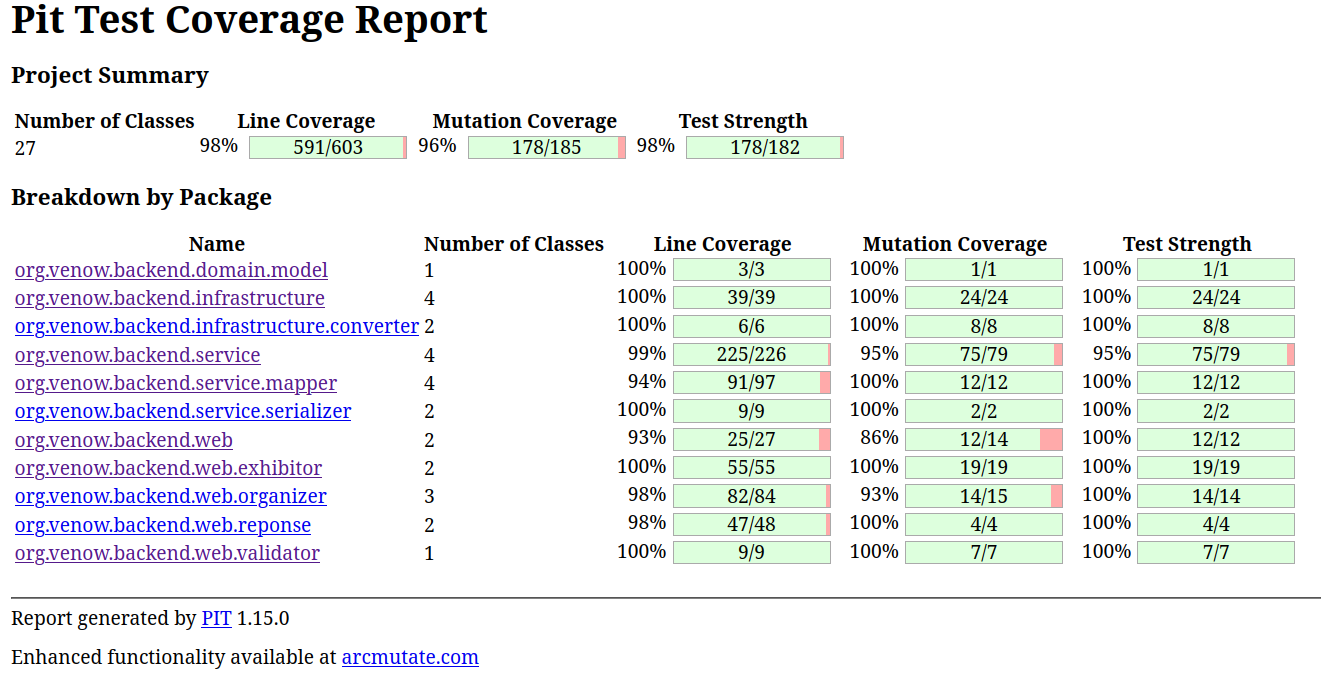
\includegraphics[width=1\textwidth]{fig/pitest-testpyramid.png}
	\caption{PIT - Mutation Testpyramid }
	\label{fig:pitest-testpyramid-full}
\end{figure}